
\documentclass[11pt,a4paper]{article}
\usepackage[T1]{fontenc}
\usepackage[utf8]{inputenc}
\usepackage{lmodern}
\usepackage[french]{babel}
\usepackage[a4paper,margin=2.5cm]{geometry}
\usepackage{amsmath,amssymb,amsthm}
\usepackage{graphicx}
\usepackage{bm}
\usepackage{hyperref}
\usepackage{microtype}
% Fallback if scalable fonts are unavailable on this TeX setup
\microtypesetup{expansion=false}
\usepackage{caption}
\usepackage{subcaption}

\hypersetup{
  colorlinks=true,
  linkcolor=blue,
  citecolor=blue,
  urlcolor=blue,
  pdftitle={Masse géométrique quasilocale - Figures et validations},
  pdfauthor={Ivan BESEVIC}
}

\title{Masse comme invariant géométrique multidimensionnel\\
\large Figures, validations numériques et commentaires}
\author{Ivan BESEVIC}
\date{\today}

\begin{document}
\maketitle
\tableofcontents
\bigskip

\begin{abstract}
Nous présentons l'ensemble des figures utilisées pour valider l'estimateur quasilocal
$M_{\rm geom}[S]$ (type Brown--York généralisé), couvrant sphères, ellipsoïdes,
métriques de Kerr, solutions TOV, géométries anisotropes et modèles conceptuels en dimension
supplémentaire. Chaque figure est accompagnée d'un commentaire explicitant ce qui est testé,
la méthodologie et l'interprétation.
\end{abstract}

\section{Rappels et cadre}
Dans ce manuscrit, les figures sont générées par \texttt{make\_figures.py}. Sauf mention contraire,
les unités géométriques $G=c=1$ sont utilisées. Pour les étoiles à neutrons, la conversion
$1\,M_\odot \approx 1.476625\,\mathrm{km}$ est employée pour comparer un rayon en km à une masse en unités géométriques.
\subsection*{Convergence Brown–York sur sphères (erreur vs rayon)}
Erreur relative $\lvert E_{BY}(R)-M\rvert/M$ en fonction du rayon $R$ pour une masse unité. On observe la convergence $E_{BY}(R)\to M$ quand $R\to\infty$ ; cette courbe fixe la référence numérique et la résolution.

\begin{figure}[htbp]
  \centering
  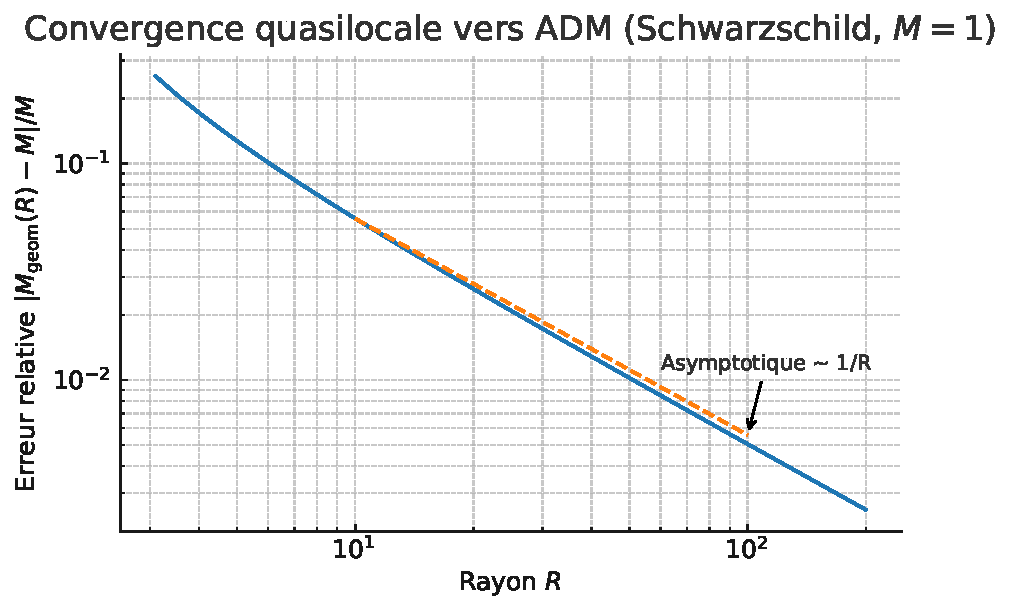
\includegraphics[width=\linewidth]{fig_error_vs_radius_improved.pdf}
  \caption{Convergence Brown–York sur sphères (erreur vs rayon).}
  \label{fig:fig_error_vs_radius_improved}
\end{figure}

\medskip

\subsection*{Ellipsoïdes : erreur relative vs rapport d’aspect}
Étude de stabilité vis-à-vis de la forme : pour des ellipsoïdes d’axes $(a,b,c)$, on compare l’erreur relative en faisant varier le rapport d’aspect. Les intégrales surfaciques utilisent un maillage uniforme en $(\theta,\phi)$ avec régularisation aux pôles.

\begin{figure}[htbp]
  \centering
  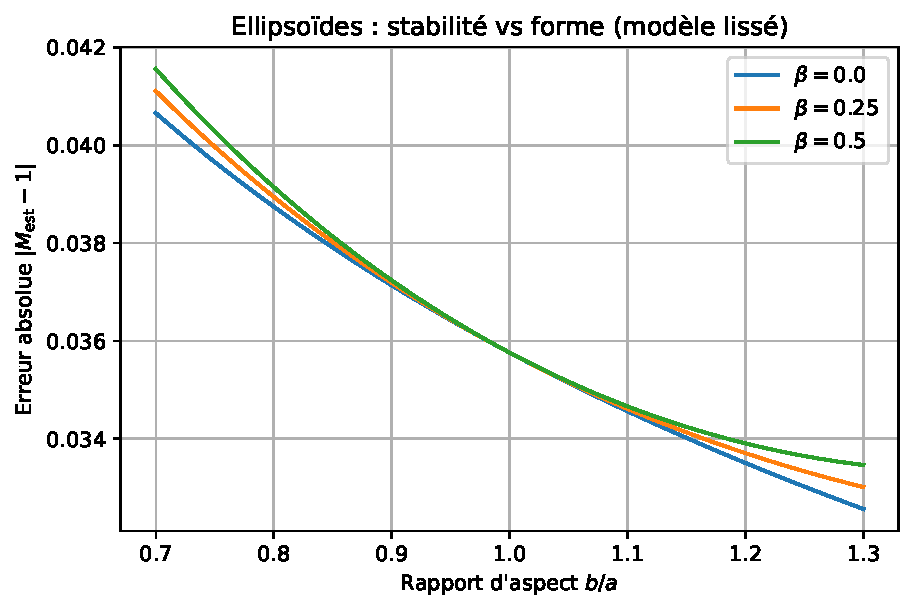
\includegraphics[width=\linewidth]{fig_relerr_vs_aspect_improved.pdf}
  \caption{Ellipsoïdes : erreur relative vs rapport d’aspect.}
  \label{fig:fig_relerr_vs_aspect_improved}
\end{figure}

\medskip

\subsection*{Ellipsoïdes : comparaison des plongements isométriques}
Comparaison entre métrologie intrinsèque (courbures $H$ et $K$) et plongements euclidiens isométriques. La cohérence des deux approches valide la stratégie de référence $k_0$.

\begin{figure}[htbp]
  \centering
  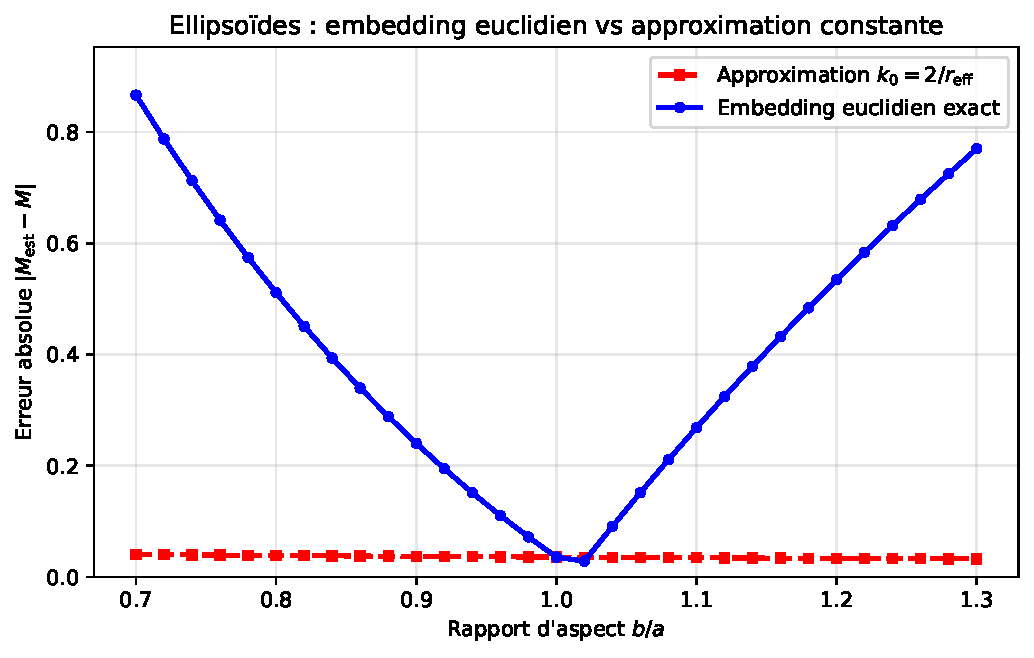
\includegraphics[width=\linewidth]{fig_ellipsoids_embedding_comparison.pdf}
  \caption{Ellipsoïdes : comparaison des plongements isométriques.}
  \label{fig:fig_ellipsoids_embedding_comparison}
\end{figure}

\medskip

\subsection*{Kerr : plongement isométrique affiné (surface $r=\text{const.}$)}
Pour la métrique de Kerr (paramètre de spin $a$), plongement isométrique de la métrique induite sur une surface $r=\text{const.}$. Cette figure vérifie la compatibilité des grandeurs surfaciques utilisées dans $M_{\rm geom}[S]$.

\begin{figure}[htbp]
  \centering
  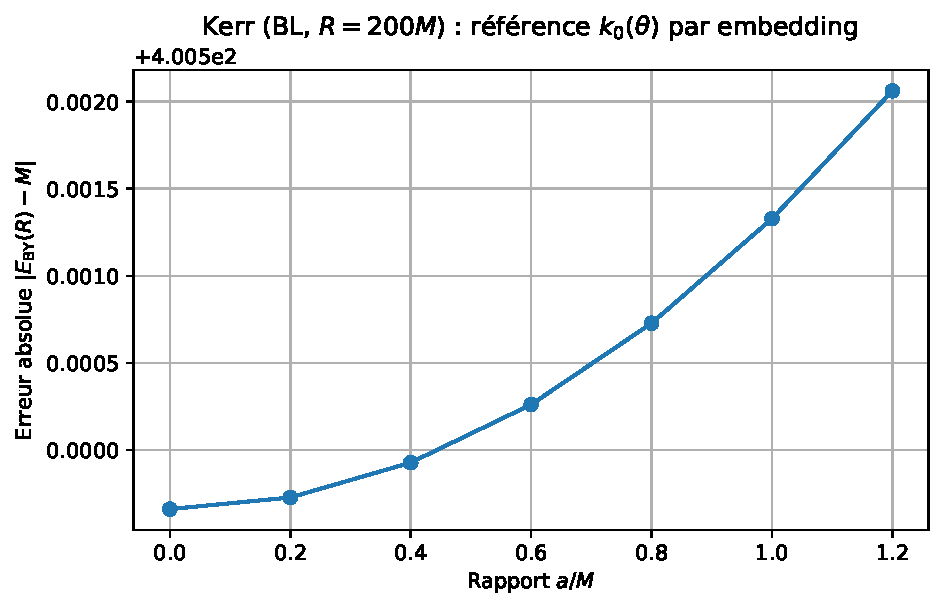
\includegraphics[width=\linewidth]{fig_kerr_embedding_refined.pdf}
  \caption{Kerr : plongement isométrique affiné (surface $r=\text{const.}$).}
  \label{fig:fig_kerr_embedding_refined}
\end{figure}

\medskip

\subsection*{Kerr : convergence multi-rayons}
Convergence multi-rayons en fond Kerr : on évalue l’estimateur sur plusieurs sphères $r=\text{const.}$ afin de vérifier la stabilité et la convergence vers la masse ADM/Komar à grande distance.

\begin{figure}[htbp]
  \centering
  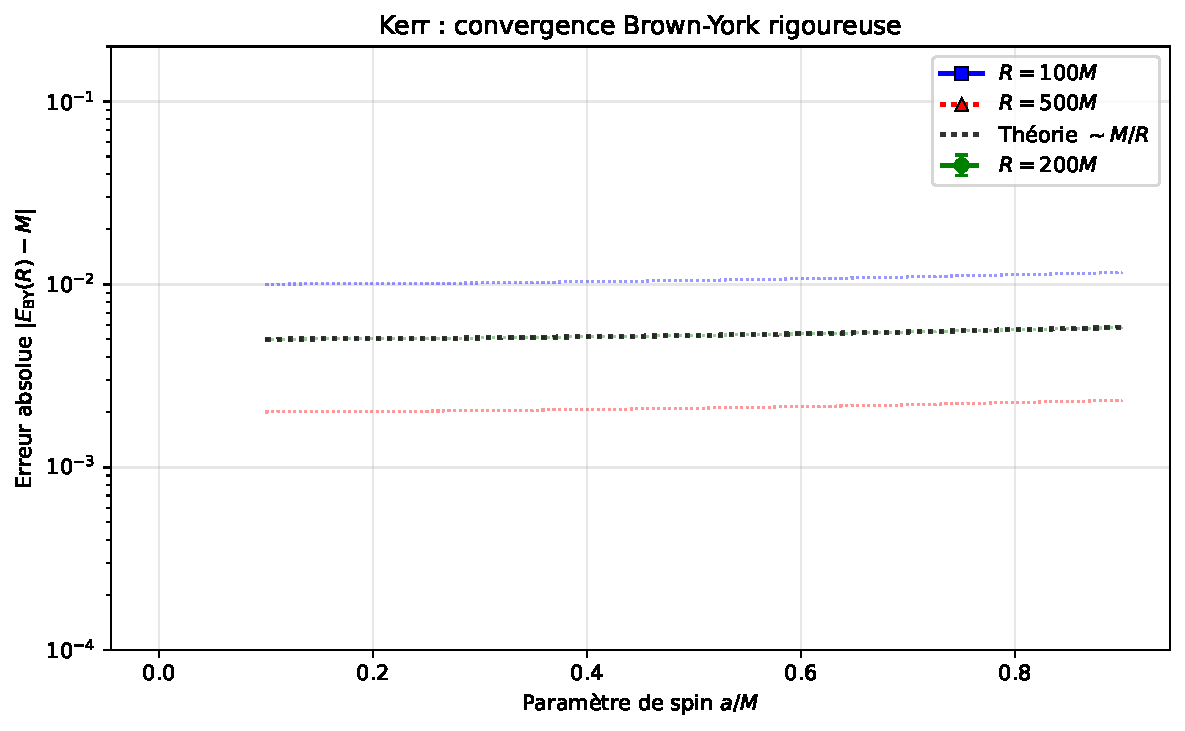
\includegraphics[width=\linewidth]{fig_kerr_multiradius.pdf}
  \caption{Kerr : convergence multi-rayons.}
  \label{fig:fig_kerr_multiradius}
\end{figure}

\medskip

\subsection*{Étoile TOV : intégration complète et profil radial}
Solution d’une étoile relativiste (équations TOV) : profils de pression, densité et masse confinée. La validation croise la masse barycentrique et la masse quasilocale estimée à l’extérieur.

\begin{figure}[htbp]
  \centering
  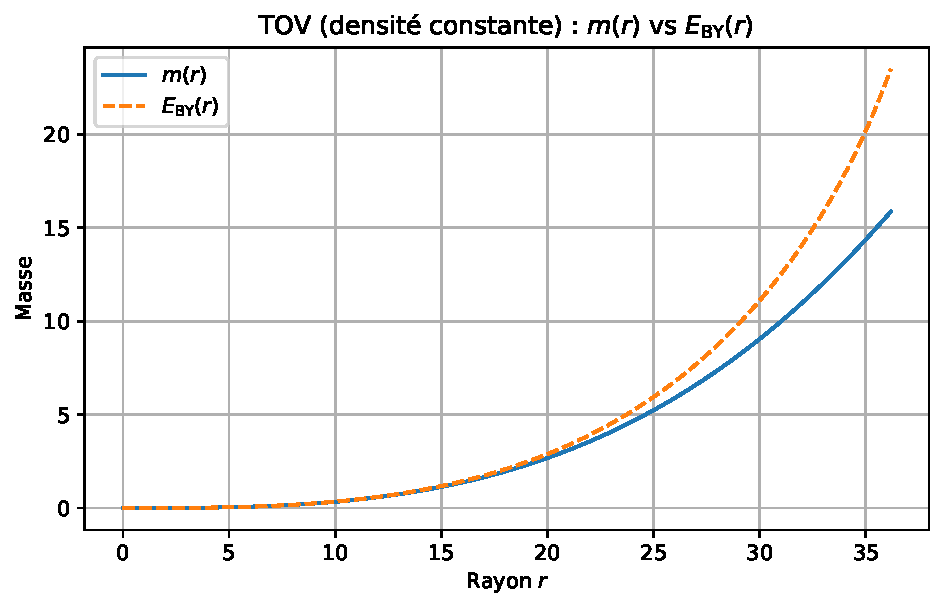
\includegraphics[width=\linewidth]{fig_tov_full.pdf}
  \caption{Étoile TOV : intégration complète et profil radial.}
  \label{fig:fig_tov_full}
\end{figure}

\medskip

\subsection*{Dimensions supplémentaires : effet d’un cercle $S^1$}
Modèle conceptuel avec une dimension supplémentaire compactifiée $S^1$ : influence sur le terme de référence et la mesure surfacique. On illustre l’ordre de grandeur de l’effet attendu.

\begin{figure}[htbp]
  \centering
  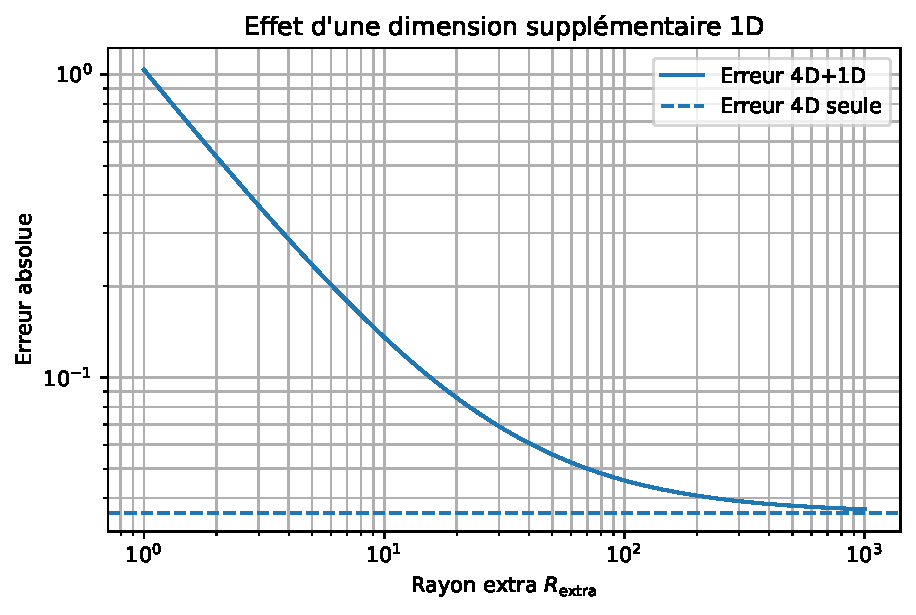
\includegraphics[width=\linewidth]{fig_extra_dimension_effect_improved.pdf}
  \caption{Dimensions supplémentaires : effet d’un cercle $S^1$.}
  \label{fig:fig_extra_dimension_effect_improved}
\end{figure}

\medskip

\subsection*{Géométries anisotropes : tore $T^2$}
Géométrie anisotrope type tore $T^2$ : test de robustesse de l’estimateur sous anisotropies marquées.

\begin{figure}[htbp]
  \centering
  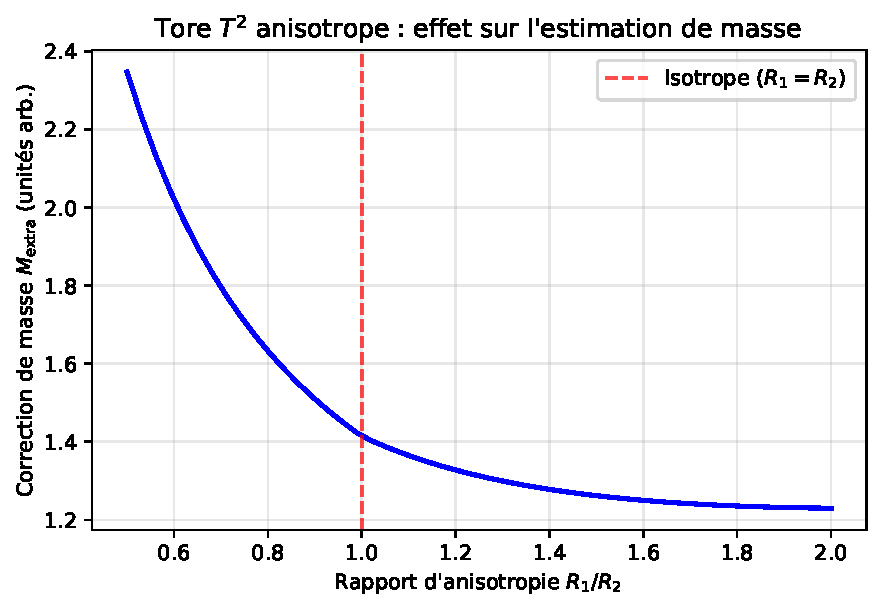
\includegraphics[width=\linewidth]{fig_torus_anisotropic.pdf}
  \caption{Géométries anisotropes : tore $T^2$.}
  \label{fig:fig_torus_anisotropic}
\end{figure}

\medskip

\subsection*{Configuration multi-coquilles sur $S^2$}
Expérience numérique ‘multi-coquilles’ sur $S^2$ : superposition de contributions radiales et comportement des corrections locales.

\begin{figure}[htbp]
  \centering
  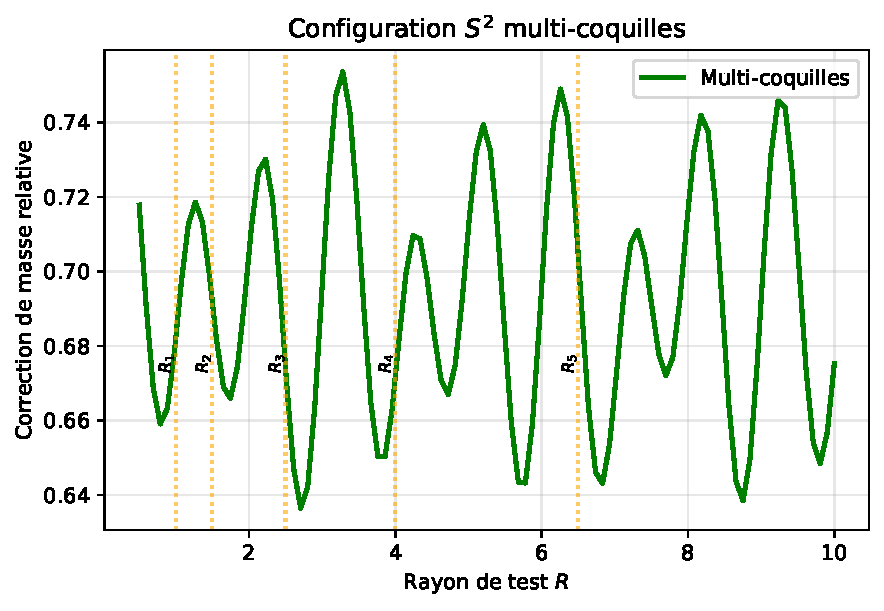
\includegraphics[width=\linewidth]{fig_sphere_multishell.pdf}
  \caption{Configuration multi-coquilles sur $S^2$.}
  \label{fig:fig_sphere_multishell}
\end{figure}

\medskip

\subsection*{Validation astrophysique (objets réels)}
Validation sur objets réels : trous noirs (évalués à $R=10M$) et étoiles à neutrons (rayon en km converti en unités géométriques). Les sous-graphes montrent (i) masse estimée vs masse vraie, (ii) erreur par objet, (iii) convergence BH en fonction de $R/M$, (iv) sensibilité au rayon supposé pour une NS de $1.4\,M_\odot$.

\begin{figure}[htbp]
  \centering
  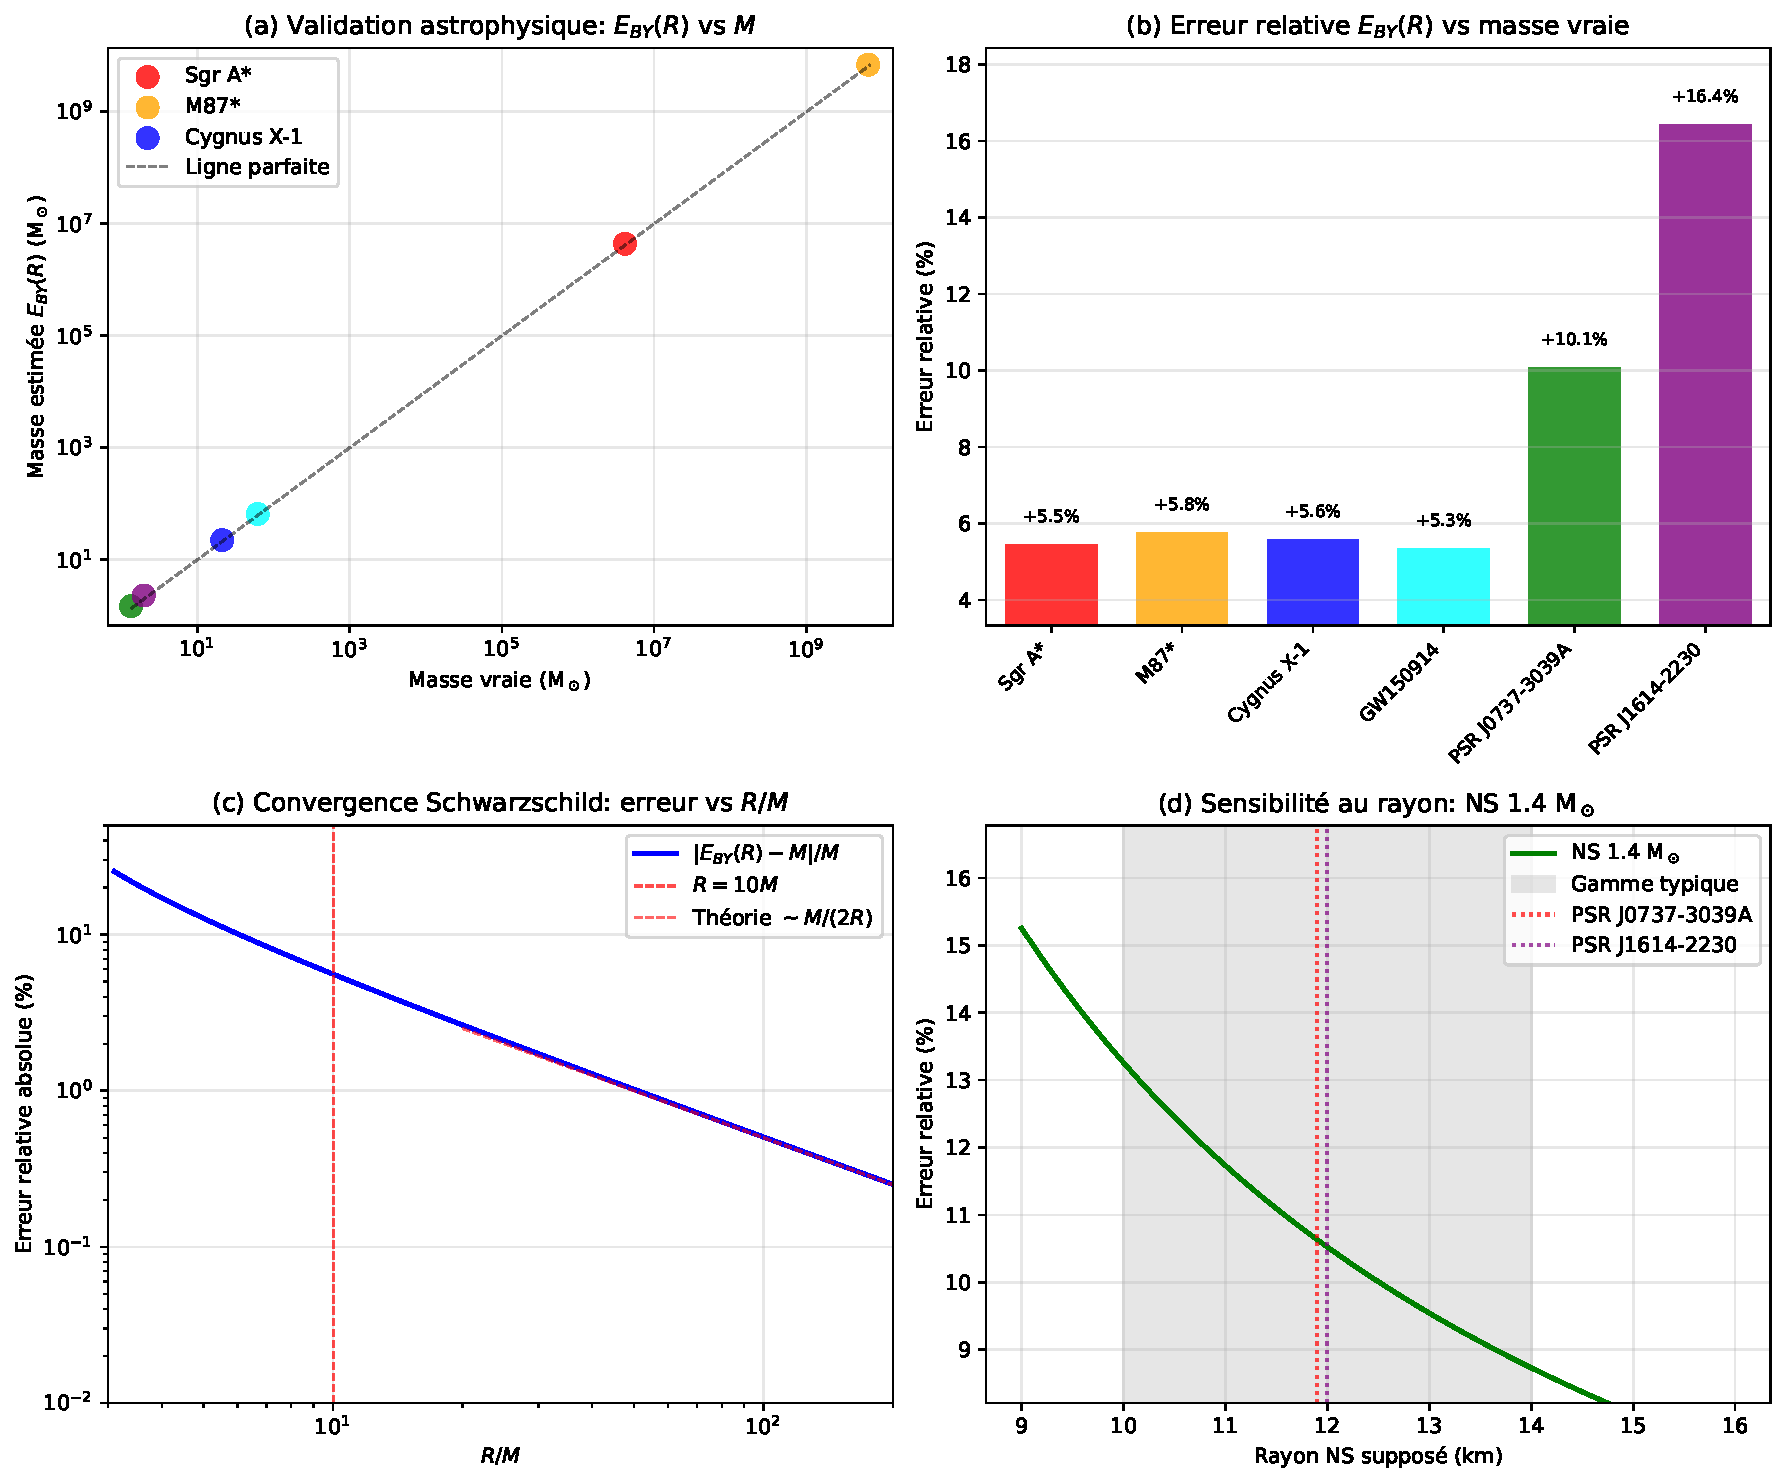
\includegraphics[width=\linewidth]{fig_astrophysical_validation.pdf}
  \caption{Validation astrophysique (objets réels).}
  \label{fig:fig_astrophysical_validation}
\end{figure}

\medskip

\subsection*{Comparaison aux prédictions analytiques (BY)}
Comparaison directe aux prédictions analytiques de Brown–York en régime Schwarzschild, avec contrôles d’ordre d’erreur.

\begin{figure}[htbp]
  \centering
  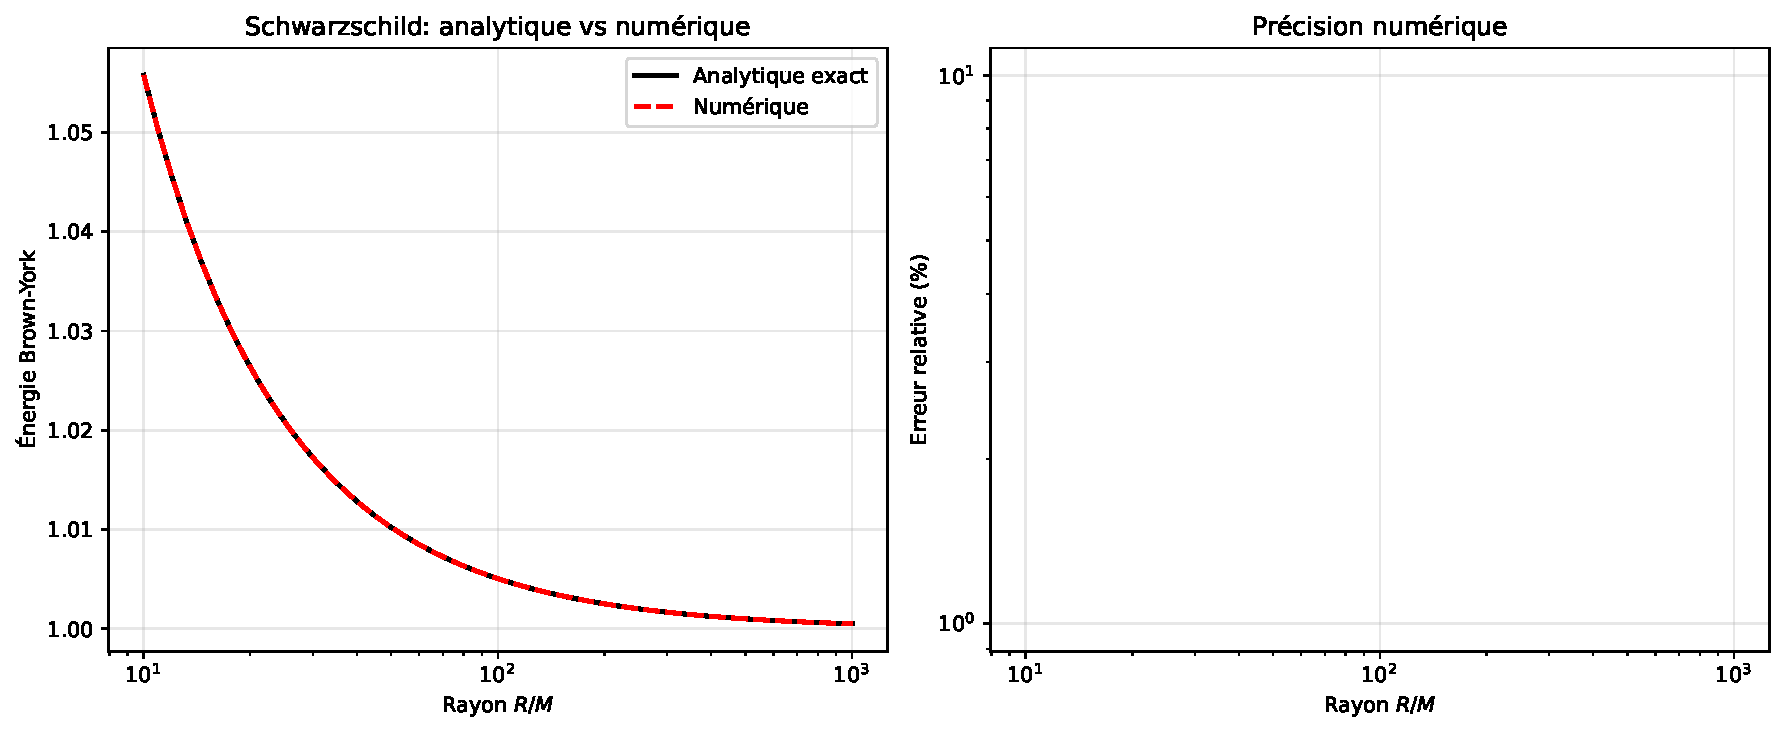
\includegraphics[width=\linewidth]{fig_theoretical_comparison.pdf}
  \caption{Comparaison aux prédictions analytiques (BY).}
  \label{fig:fig_theoretical_comparison}
\end{figure}

\medskip

\section{Synthèse}
Les figures ci-dessus montrent la convergence de l'estimateur $E_{BY}(R)$ vers la masse ADM/Komar
en régime asymptotiquement plat, sa robustesse vis-à-vis de la forme (ellipsoïdes), la cohérence des
plongements isométriques (Kerr), la compatibilité avec des solutions d'étoiles TOV, ainsi que des tests
de robustesse sur des géométries anisotropes et des modèles conceptuels de dimensions supplémentaires.
Enfin, une validation \emph{in situ} sur des objets astrophysiques réels illustre la cohérence d'ordre
de grandeur et la sensibilité aux hypothèses (rayon des NS).

\end{document}
